\documentclass{beamer}
% This is the file main.tex
\usetheme{Pittsburgh}

\usepackage{listings}


\title{Refactoring TypedData to FeatureSets using Rewriter Combinators}
\author{Clay Thomas}
\date{\today}

\begin{document}
  \begin{frame}
    \titlepage
  \end{frame}

  \begin{frame}[fragile]{The Basic Problem}
    Before:
\begin{verbatim}
  ints <- intsToTypedData <$> mkSafeHashMap
    [ ("x", someHaxlInt)
    , ("y", someOtherHaxlInt)
    ]
\end{verbatim}

    After:
\begin{verbatim}
  ints <- (toTypedData . mconcat)
    [ genFeature "x" <@ someHaxlInt
    , genFeature "y" <@ someOtherHaxlInt
    ]
\end{verbatim}
    
  \end{frame}

  \begin{frame}{Retrie Review}
    \begin{align*}
        \texttt{$\forall$ f.} & \texttt{concat $\circ$ map f} 
        & & \mapsto & & \texttt{concatMap f}
      \uncover<2->{
        \\ & 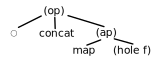
\includegraphics[height=0.1\textheight]{concatMap}
      }
      \uncover<3->{
        \\ & \texttt{(op) $\circ$ concat (ap) map (hole:f)}
      }
      \\ \texttt{$\forall$.} & \texttt{concat $\circ$ concat} 
        & & \mapsto & & \texttt{megaconcat }
      \uncover<2->{
        \\ & 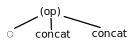
\includegraphics[height=0.065\textheight]{concatConcat}
      }
      \uncover<3->{
        \\ & \texttt{(op) $\circ$ concat concat}
      }
      \\ \texttt{$\forall$ f g.} & \texttt{first f $\circ$ second g} 
        & & \mapsto & &
      \texttt{bimap f g}
      \uncover<2->{
        \\ & 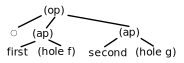
\includegraphics[height=0.1\textheight]{firstSecond}
      }
      \uncover<3->{
        \\ & \texttt{(op) $\circ$ (ap) first (hole:f)}
        \\ & \texttt{\ \ \ (ap) second (hole:g)}
      }
    \end{align*}
    
  \end{frame}

  \begin{frame}{Retrie Review}

    \begin{align*}
        \texttt{(op) $\circ$ concat (ap) map (hole:f)}
        & \mapsto & \texttt{concatMap f}
      \\ \texttt{(op) $\circ$ concat concat}
        & \mapsto & \texttt{megaconcat}
      \\ \texttt{(op) $\circ$ (ap) first (hole:f)}
      \\ \texttt{\ \ \ (ap) second (hole:g)}
        & \mapsto & \texttt{bimap f g}
    \end{align*}

    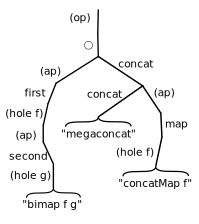
\includegraphics[height=0.5\textheight]{trieOne}
    
  \end{frame}

  \begin{frame}[fragile]{Retrie Review}
    
    \begin{columns}
      \begin{column}{0.5\textwidth}
        \begin{verbatim}
type Rewriter = EMap Template

data EMap a =
  { opEMap   :: EMap (EMap (EMap a))
        -- ^     op   lhs   rhs
  , apEMap   :: EMap (EMap a)
        -- ^    func  arg
  , varEMap  :: Data.Map String a
        -- ^            var_name
  , listEMap :: ListMap EMap a
        -- ^ => EMap (EMap (EMap (EMap ...)))
  }
        \end{verbatim}
      \end{column}
      \begin{column}{0.5\textwidth}  %%<--- here
        \begin{flushright}
        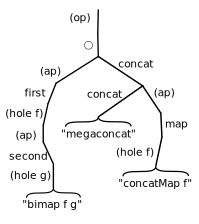
\includegraphics[width=0.6\textwidth]{trieOne}
        \end{flushright}
      \end{column}
    \end{columns}


  \end{frame}

  \begin{frame}[fragile]{Constructing New Tries}
    \begin{columns}
      \begin{column}{0.5\textwidth}
\begin{semiverbatim}
ints <- {\color<1>[rgb]{1,0,0}intsToTypedData <$> mkSafeHashMap}
    [ {\color<2>[rgb]{1,0,0} ("x", someHaxlInt)}
    , {\color<3>[rgb]{1,0,0} ("y", someOtherHaxlInt)}
    ]
\end{semiverbatim}
        \only<4>{ And more! }
      \end{column}
      \begin{column}{0.5\textwidth}  %%<--- here
        \begin{flushright}
          \only<1>{
            \includegraphics[width=0.5\textwidth]{cyclicLevel00}
          }
          \only<2>{
            \includegraphics[width=0.5\textwidth]{cyclicLevel01}
          }
          \only<3>{
            \includegraphics[width=0.5\textwidth]{cyclicLevel02}
          }
          \only<4>{
            \includegraphics[width=0.5\textwidth]{cyclicLevel03}
          }
        \end{flushright}
      \end{column}
    \end{columns}
  \end{frame}

  \begin{frame}[fragile, t]{Constructing New Tries}
    \begin{columns}
      \begin{column}{0.5\textwidth}
\begin{semiverbatim}
thenApply' :: EMap a -> EMap b -> EMap (a,b)
thenApply' func arg = EMap \{ apEMap = root \}
  where {\color<2>[rgb]{1,0,0}
    root = fmap catArg func
    catArg a = fmap (a,) arg
}

thenApply :: EMap Template 
  -> EMap Template -> EMap Template
thenApply x y 
  = fmap catTemplates \$ thenApply' x y
  where
    catTemplates :: Template -> Template
      -> Template
\end{semiverbatim}
      \end{column}
      \begin{column}{0.5\textwidth}  %%<--- here
        \begin{flushright}
          \includegraphics[width=0.5\textwidth]{cyclicLevel01}
        \end{flushright}
      \end{column}
    \end{columns}
  \end{frame}


  \begin{frame}[fragile, t]{Constructing New Tries}
    \begin{columns}
      \begin{column}{0.5\textwidth}
\begin{semiverbatim}
cyclicize' :: EMap a -> EMap [a]
cyclicize' emap = reverse <$> list
  where
    list = EMap \{ listEMap = root \}
    root = ListMap
      \{ nil = [[]] {\color<2>[rgb]{1,0,0}
      , cons = fmap catRoot emap \}
    catRoot a = fmap (a:) root
}

cyclicize :: EMap Template -> EMap Template
cyclicize = fmap consTemplates . cyclicize'
  where
    consTemplates :: [Template] -> Template
\end{semiverbatim}
      \end{column}
      \begin{column}{0.5\textwidth}  %%<--- here
        \begin{flushright}
          \only<1>{
            \includegraphics[width=0.5\textwidth]{cyclicOneLevel03}
          }
          \only<2>{
            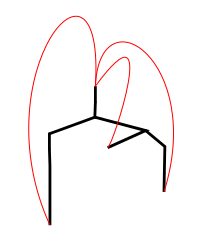
\includegraphics[width=0.5\textwidth]{cyclicRedLevel}
          }
        \end{flushright}
      \end{column}
    \end{columns}
  \end{frame}

  \begin{frame}[fragile]{They Work Kinda!}
\begin{semiverbatim}
\{-# RULES
  "outer" (fmap intsToTypedData . mkSafeHashMap) 
    = (toTypedData . mconcat)
  "inner" forall x y. (x,y) = genFeatureInt x <@ y
#-\}
... (rule loading, file shuffling)
applyRewriter \$ outer `thenApply` cyclicize inner
\end{semiverbatim}
  \end{frame}

  \begin{frame}[fragile]{They Work Kinda!}
\begin{semiverbatim}
\{-# RULES
  "outerInt" (fmap intsToTypedData . mkSafeHashMap) 
    = (toTypedData . mconcat)
  "outerBool" (fmap boolsToTypedData . mkSafeHashMap) 
    = (toTypedData . mconcat)
  ...
  "innerInt" forall x y. (x,y) = genFeatureInt x <@ y
  "innerBool" forall x y. (x,y) = genFeatureBool x <@ y
  ...
#-\}
... (rule loading, file shuffling)
applyRewriter . fold 
  \$ zipWith thenApply outers (map cyclicize inners)
\end{semiverbatim}
  \end{frame}

  \begin{frame}[fragile]{Impact}
    \begin{enumerate}
      \item Help teams transition to FeatureSet
      \item Reduce technical debt
      \item 25K lines of code
      \item Reduced usage by 2/3
    \end{enumerate}
  \end{frame}

  \begin{frame}[fragile]{Other Applications}
    \begin{enumerate}
      \item Squashing lists of lists
        \begin{verbatim}flatten' :: EMap a -> EMap b -> EMap [[b]] \end{verbatim}
      \item Collecting and moving list elements?
        \begin{verbatim}collect' :: EMap a -> EMap b -> EMap [([a],[b])] \end{verbatim}
      \item Refactoring every element in a `do` block?
    \end{enumerate}
  \end{frame}

  \begin{frame}[fragile]{It Kinda Doesn't Work}
    \begin{enumerate}
      \item Holes overlap
      \item Formatting
    \end{enumerate}
  \end{frame}
\end{document}
